\scanpage{49}
- \mspage{2} -

\margin{en fait il est \unsure{isom.} à $\widetilde M$ !}
Il en résulte que $\operatorname{Ker}(\widetilde v)$ est plat et que $\widetilde M\times_SG/\operatorname{Ker}(\widetilde v)$ est lisse. Par ailleurs, vu le choix de $\widetilde M$, Le groupe $M\times_SG/\widetilde M\times_SG=M/\widetilde M$ est étale, donc $M\times_SG/\operatorname{Ker}(\widetilde v)$ est lisse, comme extension de groupes lisses. On a évidemment $\operatorname{Ker}(\widetilde v)\subset P$, de sorte que $M\times_SG/P$ est \deleted{bien} lisse, comme quotient d'un groupe lisse.

Démonstration du théorème. L'unicité du prolongement est claire. Comme la propriété néronienne de $G$ est conservée par passage à l'hensélisé, on peut supposer $S$ hensélien. Quitte alors à remplacer $\underset{\sim}{H}$ par sa partie connexe, on peut, compte tenu du lemme 1, supposer \deleted{$\unsure{H}$} $\underset{\sim}{H}$ connexe.

a) Cas où $G$ est semi-stable. Soit $\underset{\sim}{G}_\eta$ le groupe p-divisible défini par $G_\eta$ et soit $\underset{\sim}{G}'$ le S-groupe p-divisible obtenu à partir du Schéma en groupes $G^0$.
\figure{\begin{tikzpicture}\node[draw,ellipse] {On sait};\end{tikzpicture}}
que $\underset{\sim}{G}''_\eta=\underset{\sim}{G}_\eta/\underset{\sim}{G}'_\eta$ est \inserted{un} groupe p-divisible \deleted{non-ramifié} \inserted{étale} sur $S$, \deleted{donc} \inserted{et} se prolonge en un S-groupe p-divisible, $\underset{\sim}{G}''$, étale sur $S$. D'après \uuline{Tate}, le morphisme composé $v_\eta:\underset{\sim}{H}_\eta\xrightarrow{u_\eta}\underset{\sim}{G}_\eta\longrightarrow\underset{\sim}{G}''_\eta$ se prolonge en un S-morphisme $v:\underset{\sim}{H}\longrightarrow\underset{\sim}{G}''$. Comme $\underset{\sim}{H}$ est connexe et $\underset{\sim}{G}''$ étale, $v$ est nul. \deleted{\unsure{P}} Il en résulte que $u_\eta$ se factorise à travers $\underset{\sim}{G}'_\eta$, donc toujours d'après \uuline{Tate}, se pro-longe en un S-morphisme $u:\underset{\sim}{H}\longrightarrow\underset{\sim}{G}'$ c.q.f.d.
\margin{``\unsure{donc}'' abusif \uline{OK}}
\figure{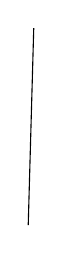
\begin{tikzpicture}\draw (0,0)--(.07,2.5);\end{tikzpicture}}

b) Cas général.
\figure{\begin{tikzpicture}\node[draw,rounded corners] (a) {On sait};\node[draw,ellipse,align=left] (b) at (-4,-1) {? Cas où $G_\eta$ est une\\V.A. seulement!};\node at (-4,-2) {OK};\draw (b.north east)..controls(-2.2,.4)..(a.west);\end{tikzpicture}}
qu'il existe une extension de traits $S'\longrightarrow S$, finie et plate, telle que, si $\eta'$ est le point générique de $S'$, le $S'$ modèle de Néron $\mathcal G'$ de $G_{\eta'}$ soit semi\inserted{-}stable. D'après a), le morphisme $u_{\eta'}:\underset{\sim}{H}_{\eta'}\longrightarrow G_{\eta'}$ se prolonge en un $S'$-morphisme $u':\underset{\sim}{H}_{S'}\longrightarrow\mathcal G'$. Rappelons que le $S$-modèle de Néron de $G_\eta$, c'est à dire $G$, s'obtient à partir de $\mathcal G'$ de la façon suivante (cf. note sur les modèles de Néron prop. 2.5):

On considère le S-groupe S-néronien $\mathcal G=\prod_{S'/S}(\mathcal G'/S')$. Le groupe $G_\eta$ s'identifie canoniquement à un sous-groupe de $\mathcal G_\eta$; soit $G_1$ l'adhérence schématique dans $\mathcal G$ de $G_\eta$. Alors $G$ est le ``lissifié '' de $G_1$.

\mspage{48}
